\documentclass[format=acmlarge]{acmart}

\usepackage{amsmath}
\DeclareMathOperator*{\argmax}{argmax}

\usepackage{hyperref}

\setcopyright{rightsretained}
\copyrightyear{2017}

\begin{document}
\title{Using support vector machine techniques to correlate past and future large-cap stock returns}

\author{Kenneth Allen}
\affiliation{%
  \institution{Armstrong State University}
  \department{Department of Computer Science \& Information Technology}
  \city{Savannah}
  \state{GA}
  \postcode{31419}
  \country{United States of America}}
\email{ka3878@stu.armstrong.edu}

\author{Jeffrey Young}
\affiliation{%
  \institution{Armstrong State University}
  \department{Department of Computer Science \& Information Technology}
  \city{Savannah}
  \state{GA}
  \postcode{31419}
  \country{United States of America}}
\email{jy8672@stu.armstrong.edu}

\begin{abstract}
Quantitative analysis of the stock market to predict future behavior has long been a very active area of study with clear applicability, both for profit-seeking and informing macroeconomic policy.  We apply support vector machine techniques to show that simple daily total return data can be shown to be correlated with future performance.  Although our method is not immediately applicable for predicting beyond the current moment in time, it demonstrates that the potential for such models does exist.
\end{abstract}

\keywords{Machine learning, Support Vector Machines, LibSVM, Stock prediction, S\&P 500}

\maketitle

\section{Data Processing}
\begin{figure}
  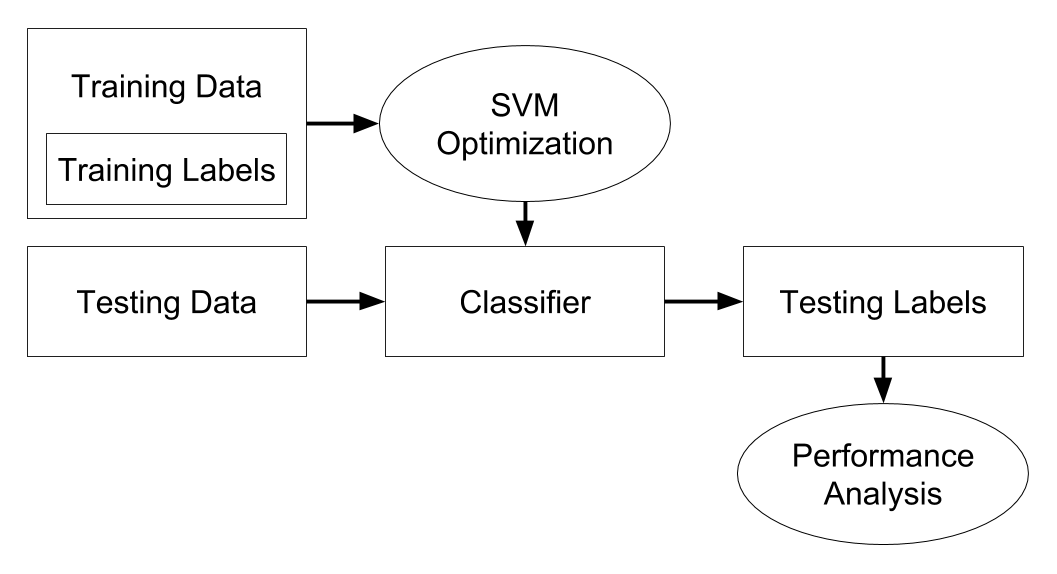
\includegraphics{block-diagram}
  \caption{Block diagram of classifier system.}
  \label{fig:one}
\end{figure}

\subsection{Data}
The economics department of Armstrong State University has a dataset spanning over 16 years of daily total returns for each stock listed in the Standard \& Poor's 500 Index, which consists of 505 stocks from 500 of the largest companies in the world, measured by total market capitalization.  We were given limited access to this data to perform the experiments for this project.  The data takes the form of dated percentage daily total returns and occupies about 23.8 mibibytes (25 million bytes).

For each test, 10\% of the data was randomly removed and used as a test set while the remaining 90\% was used as a training set.

\subsection{Training Labels}
Labels for this undertaking were calculated from the excluded data from the test period, which was chosen as the final year of the data:  March 22, 2016, to March 21, 2017.  Each stock was labeled with whether its total return exceeded that of the S\&P 500 index during that period.

\subsection{Classifier}
Our system uses the LibSVM library to implement SVM training and classification.  It interacts with its programmatic Java API to add features like statistics tracking and training models with different parameters across different threads.  Parameters were evaluated at multiple values from ranges recommended by the LibSVM authors.

\subsection{Prediction}
Prediction quality was measured with a bevy of statistics.  Accuracy is simple to calculate ($\frac{\textrm{correct classifications}}{\textrm{tested elements}}$).

For binary criteria, more informative values can be generated.  Use $\mathit{TP}$, $\mathit{FP}$, $\mathit{FN}$, and $\mathit{TN}$, to represent true positives, false positives, false negatives, and true negatives, respectively.  Especially important are true positive rate ($\mathit{TPR} = \frac{\mathit{TP}}{\mathit{TP} + \mathit{FN}}$), true negative rate ($\mathit{TNR} = \frac{\mathit{TN}}{\mathit{FP} + \mathit{TN}}$), positive predictive value ($\mathit{PPV} = \frac{\mathit{TP}}{\mathit{TP} + \mathit{FP}}$), and negative predictive value ($\mathit{NPV} = \frac{\mathit{TN}}{\mathit{FN} + \mathit{TN}}$).  ``AUC'' and $F_1$ score are discussed below.

\begin{figure}
  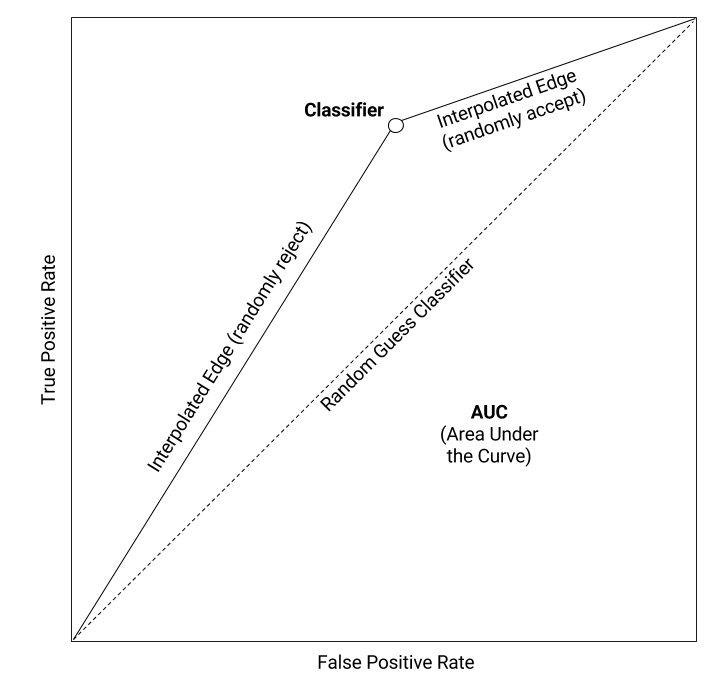
\includegraphics{interpolated-roc}
  \caption{Interpolated Receiver Operating Characteristic.}
  \label{fig:two}
\end{figure}

Traditional two-class SVM does not have a sensitivity parameter, so it only creates one point on a Receiver Operating Characteristic (ROC) graph.  We can trivially interpolate between that point and the points $(0, 0)$ and $(1, 1)$ by imagining a series of classifiers that randomly choose with a certain probability whether to refer to our classifier or to automatically reject or accept, respectively (as in Fig. 2).  (This is equivalent to `convex hull' techniques, but for a single data point.)  In this way, we get a curve and can calculate the area under it simply as $\mathit{AUC} = \frac{\mathit{TPR} + \mathit{TNR}}{2}$.  The $F_1$ score is calculated as the harmonic mean of $\mathit{TPR}$ and $\mathit{PPV}$:

$$F_1 = \frac{2}{\frac{1}{\mathit{TPR}} + \frac{1}{\mathit{PPV}}}$$

\section{Results and Performance}

\begin{table}
  \caption{Classifier results: top 5 ROC-AUC.}
  \label{tab:one}
  \begin{tabular}{ll|lll|ll}
    $C$ & Kernel & Accuracy & ROC-AUC & $F_1$ score & \# Selected & Simulated Return\\
    \hline
    0.25 & polynomial (degree 4) & 0.820 & 0.821 & 0.824 & 25 & 35.6\%\\
    0.5 & polynomial (degree 3) & 0.820 & 0.821 & 0.824 & 25 & 36.0\%\\
    2 & polynomial (degree 4) & 0.820 & 0.819 & 0.830 & 27 & 34.3\%\\
    1 & polynomial (degree 2) & 0.820 & 0.819 & 0.830 & 27 & 35.6\%\\
    1 & polynomial (degree 4) & 0.820 & 0.819 & 0.830 & 27 & 34.3\%\\
  \end{tabular}
\end{table}

Table 1 gives performance statistics for different parameterizations of the classifier, chosen for the best ``area under the curve'' (for their interpolated receiver operating characteristic).  Since every polynomial polynomial degree between 2 and 10 was tested, we see that quadratic, cubic, and quartic kernels give better results than a linear kernel, higher-degree polynomial kernels, or radial-basis function kernels.  Also, a clear bias toward lower $C$ values is observed.  Each of these classifiers selected about half of the test set of size 50 to beat the market average, which is in line with expectations.

\begin{table}
  \caption{Classifier results: top 5 simulated returns.}
  \label{tab:two}
  \begin{tabular}{ll|lll|ll}
    $C$ & Kernel & Accuracy & ROC-AUC & $F_1$ score & \# Selected & Simulated Return\\
    \hline
    0.25 & radial-basis ($\gamma = 0.2$) & 0.520 & 0.538 & 0.143 & 2 & 66.8\%\\
    0.5 & radial-basis ($\gamma = 0.1$) & 0.620 & 0.635 & 0.424 & 7 & 62.0\%\\
    0.25 & radial-basis ($\gamma = 0.5$) & 0.500 & 0.518 & 0.138 & 3 & 50.3\%\\
    1 & radial-basis ($\gamma = 0.1$) & 0.580 & 0.591 & 0.432 & 11 & 44.9\%\\
    0.5 & radial-basis ($\gamma = 0.2$)& 0.580 & 0.591 & 0.432 & 11 & 44.9\%\\
  \end{tabular}
\end{table}

Table 2 shows the top-performers ranked by simulated return, which is calculated by imagining the total return (over the test period) for an investment split equally between each of the stocks the classifier recommended.  We see a much different trend, where the highest possible returns are delivered by classifiers that managed to select very few stocks that each performed excellently.  These classifiers are all based on radial-basis functions with low $\gamma$ and $C$ values.  Further research could help determine why radial-basis function kernels are uniquely suited to fixating on high-performing outliers on our dataset.

\begin{table}
  \caption{Example classification of test set ($C = 0.25$, quartic kernel).}
  \label{tab:three}
  \begin{tabular}{ll|ll|ll}
KR & -24.1\%   & \textbf{WU} & 10.9\%    & \textbf{AIZ} & 25.4\%\\
MAT & -21.5\%  & NEM & 12.8\%   & \textbf{NOC} & 26.1\%\\
KIM & -17.4\%  & FBHS & 14.4\%  & \textbf{HOG} & 28.1\%\\
HRB & -13.1\%  & HD & 15.9\%    & CBG & 28.5\%\\
BMY & -12.6\%  & BEN & 17.2\%   & \textbf{QRVO} & 29.5\%\\
DLTR & -10.5\% & \textbf{HON} & 17.5\%   & \textbf{COO} & 30.6\%\\
SBUX & -7\%    & CVX & 17.5\%   & \textbf{CTXS} & 30.9\%\\
AAP & -5.9\%   & \textit{S\&P 500} & 17.5\% & MPC & 35.9\%\\
DISCA & -1.9\% & \textbf{BWA} & 17.8\%   & \textbf{YHOO} & 36.4\%\\
\textbf{GE} & 0.3\%     & \textbf{LLY} & 19.5\%   & ATVI & 45.5\%\\
VRTX & 3.7\%   & FTV & 20\%     & \textbf{ULTA} & 48.2\%\\
ES & 5.2\%     & \textbf{CCL} & 20.1\%   & \textbf{PRU} & 54.5\%\\
WLTW & 6.6\%   & \textbf{MCO} & 20.3\%   & \textbf{WDC} & 59.9\%\\
CHRW & 8.2\%   & KHC & 20.7\%   & \textbf{LRCX} & 61.1\%\\
UPS & 8.4\%    & \textbf{KMX} & 23.2\%   & \textbf{ZION} & 72.6\%\\
\textbf{LVLT} & 8.7\%   & \textbf{ARNC} & 24.2\%  & \textbf{CSX} & 79.8\%\\
FOXA & 9.3\%   & \textbf{CELG} & 24.7\%  & \textbf{MU} & 118.8\%\\
  \end{tabular}
\end{table}

Table 3 gives the specific results from the top-performing configuration ranked by ROC-AUC, as in Table 1.  The stocks are sorted by increasing return during the test period, and those that were predicted to outperform the S\&P 500 index have their tickers bolded.  The few false positives (GE, LVLT, WU, and HON) are plainly visible, as are the false negatives (FTV, KHC, CBG, MPC, and ATVI).  The index itself is italicized in approximately the middle of the list, where one would expect it.

\section{Discussion}
\subsection{Applications}
Although we used `foreknowledge' of the test period to train our model, these results do demonstrate that stocks that will outperform the market in the future could have similarities in their past performance that machine learning techniques can discuss.  One application of this would be for someone with expert knowledge or insider information to label a training set of stocks.  SVM optimization would create a model that could evaluate whether other stocks are `like' the expert's picks.  Another application could be to time-shift data and see if there are recognizable patterns in daily returns that repeat over intervals, which could potentially be projected into the future.

\subsection{Conclusion}
Machine learning techniques can be used to distinguish effectively between large-cap stocks that will and will not outperform the market over a specific period of time.  SVM is particularly well-suited to this task because of its configurability and ability to effectively process large training sets with large numbers of features.  Although our model was constructed using foreknowledge of stocks' performance, other, less absolute methods could be used to label training data for the same or similar purposes.

\section{Works Cited}
\begin{itemize}
\item Ben-Hur, A., \& Weston, J. \textit{A User's Guide to Support Vector Machines}. Retrieved from http://pyml.sourceforge.net/doc/howto.pdf
\item Gavrilov, Z. \textit{SVM Tutorial}. Retrieved from http://web.mit.edu/zoya/www/SVM.pdf
\item Chang, C., \& Lin, C. \textit{LIBSVM: A Library for Support Vector Machines}. Retrieved from https://www.cs.nmt.edu/~kdd/libsvm.pdf
\item Smith, B. T. \textit{Lagrange Multipliers Tutorial in the Context of Support Vector Machines}. Retrieved from http://www.engr.mun.ca/~baxter/Publications/LagrangeForSVMs.pdf
\end{itemize}

\end{document}